\documentclass[11pt]{article}

\usepackage[letterpaper,margin=0.95in]{geometry}
\usepackage{amsmath,amssymb,mathtools}
\usepackage{booktabs}
\usepackage{enumitem}
\usepackage{graphicx}
\usepackage{hyperref}
\usepackage{microtype}
\usepackage{xcolor}
\usepackage{url}

\hypersetup{
  colorlinks=true,
  linkcolor=black,
  citecolor=blue!55!black,
  urlcolor=blue!55!black
}

\setlength{\parindent}{0pt}
\setlength{\parskip}{0.43em}
\setlist[itemize]{leftmargin=1.25em,itemsep=0.12em,topsep=0.12em}
\setlist[enumerate]{leftmargin=1.4em,itemsep=0.12em,topsep=0.12em}
\renewcommand{\arraystretch}{1.08}

\newcommand{\base}{\mathrm{b}}
\newcommand{\qasset}{\mathrm{q}}
\newcommand{\cash}{\mathrm{cash}}
\newcommand{\live}{\mathrm{live}}
\newcommand{\hlp}{\mathrm{hLP}}
\newcommand{\ylp}{\mathrm{yLP}}
\newcommand{\debt}{\mathrm{debt}}
\newcommand{\nad}{\mathrm{NAD}}
\newcommand{\bps}{\mathrm{bps}}

\title{\vspace{-1.4em}Omnipair Dusk: An Oracle-less Generalized AMM for Lending, Swaps, and Leveraged Liquidity}
\author{
  Omnipair Contributors\\[-0.25em]
  \small Technical draft for Omnipair Dusk v2\\[-0.25em]
  \small \url{https://github.com/omnipair}
}
\date{Draft, July 2026}

\begin{document}
\maketitle
\vspace{-1.2em}

\begin{abstract}
Omnipair Dusk is an oracle-less market primitive on Solana that joins constant-product exchange, isolated lending, yield-bearing liquidity, and leveraged LP vaults inside one accounting system. A Dusk market prices swaps from its own reserves, values credit risk from cached in-protocol references, and routes losses through market-local buffers. The central object is a live reserve coordinate
\[
R_{\live,i}=R_{\cash,i}+D_{\cash\text{-}\debt,i}+R_{\hlp,i},
\]
which extends the usual automated market maker reserve by separating withdrawable cash, cash-backed debt, and synthetic hLP live depth. This note gives a compact model of Dusk's reserve invariant, explains why ordinary borrow activity need not move spot price, and shows how hLP can change depth while preserving the spot coordinate. It then places Dusk's leveraged-liquidity design next to Yield Basis and Morpho-style adaptive rates, and reports small deterministic simulations for rate adaptation, slippage depth, and hLP tracking error.
\end{abstract}

\textbf{Disclaimer.} This paper is for technical discussion only. It describes experimental smart-contract mechanisms and does not constitute investment, legal, tax, accounting, or financial advice. Dusk v2 is unaudited and under active development.

\section{Introduction}

Most onchain leverage systems separate three functions that are naturally coupled: spot liquidity, borrowable liquidity, and liquidation liquidity. Spot automated market makers hold inventory; lending markets maintain collateral and debt books; liquidation agents bridge the two under stress. This separation is workable for liquid, whitelisted assets, but it is poorly matched to long-tail markets where liquidity is fragmented and external price feeds are expensive, delayed, or unavailable.

The practical demand is not small. A public Omnipair analysis notebook sampling the top 3000 Raydium pairs by 24-hour volume found that 78.41\% of sampled volume was in pairs below \$100M fully diluted valuation and roughly 94.82\% below \$1B \cite{omnipair-raydium-notebook}. These figures are not a proof that every long-tail asset should be marginable. They are evidence that a large share of trading demand lives outside the set of assets that oracle-governed lending venues can list quickly.

Dusk follows the Generalized Automated Market Maker (GAMM) thesis: a pair-local AMM can be the source of both price discovery and credit constraints \cite{omnipair-docs-intro,omnipair-docs-gamm}. Liquidity providers deposit both sides of a pair, traders swap against the same reserve coordinate, and borrowers use one side as collateral to borrow the other. Since valuation is derived from in-market state rather than an external oracle, each market can be isolated. Failure in one pair does not need to contaminate other pairs. In form, this paper follows recent protocol whitepapers that state the accounting model directly before implementation details \cite{morpho-midnight}.

The v2 contribution is not merely adding features to an AMM. It is a stricter reserve accounting model that makes three flows coexist:
\begin{enumerate}
  \item normal LP liquidity, represented by yield-bearing yLP shares;
  \item cash-backed borrowing, which removes cash but leaves the live price coordinate unchanged;
  \item hLP vaults, which target one-sided leveraged LP exposure by adding explicit synthetic live depth and funding debt.
\end{enumerate}

The paper is intentionally compact. It omits program accounts and instruction details unless they alter the mechanism. The goal is to state the invariant, the risk model, and the economic contrast clearly enough that an implementer or reviewer can reason about the design without reading a protocol manual.

\section{Market Model}

A Dusk market is a pair $(\base,\qasset)$ with side-specific accounting. For each side $i\in\{\base,\qasset\}$, the market records:

\begin{center}
\begin{tabular}{ll}
\toprule
Symbol & Meaning \\
\midrule
$R_{\cash,i}$ & withdrawable cash reserve in the market vault \\
$D_{\cash\text{-}\debt,i}$ & cash-backed outstanding debt on side $i$ \\
$R_{\hlp,i}$ & hLP-owned synthetic live reserve depth \\
$R_{\live,i}$ & reserve coordinate used for swaps and spot price \\
$S_{\ylp}$ & normal two-sided LP share supply \\
$D_{\hlp,i}$ & hLP funding debt on side $i$ \\
\bottomrule
\end{tabular}
\end{center}

Spot price is read from live reserves. With quote as numeraire,
\begin{equation}
P_{\base\to\qasset}=\frac{R_{\live,\qasset}}{R_{\live,\base}}.
\end{equation}
Swaps use the constant-product coordinate
\begin{equation}
K=R_{\live,\base}R_{\live,\qasset},
\end{equation}
with fees accounted outside the principal claim before being routed through yield indexes.

yLP represents a floating two-sided claim on principal reserves. If fees and interest are denoted by growth indexes rather than auto-compounded into principal, the yLP claim remains simple:
\begin{equation}
\mathrm{claim}_{i}(s)=s\cdot\frac{R_{\live,i}}{S_{\ylp}},
\end{equation}
subject to cash availability when a withdrawal actually moves tokens out of the vault. This distinction is central: a live reserve may quote depth, but only cash can settle a transfer.

hLP represents an aggregate leveraged LP vault. A base hLP vault receives base, funds the quote leg, receives yLP exposure, and tracks debt against the funded side. A quote hLP vault is symmetric. hLP is therefore neither a normal LP share nor a borrower position. It is a market-level transformation of depth, debt, and NAV.

The design uses three separate notions of value. Principal reserve value determines share accounting. Cash value determines whether tokens can leave the vault. Risk value determines whether debt can be opened or must be closed. Many AMM and lending bugs come from collapsing these three quantities into one balance. Dusk keeps them separate even when they happen to be numerically equal in a quiet market.

Yield is also deliberately non-compounding at the principal layer. Swap fees and realized borrow interest are recorded in side-specific vaults and distributed through growth indexes. This makes the principal invariant easier to audit: ordinary yield is a liability owed to share holders, not an unlabelled increase in the reserves from which new LP shares are minted. In symbols, if $G_i$ is the cumulative growth index for side $i$, a yLP account earns by checkpointing $s(G_i-G_i^{\mathrm{last}})$, while its principal claim remains defined by reserve shares.

\section{The GAMM Invariant}

Dusk's reserve equation is
\begin{equation}
\boxed{R_{\live,i}=R_{\cash,i}+D_{\cash\text{-}\debt,i}+R_{\hlp,i}.}
\label{eq:live}
\end{equation}
Without hLP, $R_{\hlp,i}=0$, and the equation reduces to the v1 GAMM relation between cash and borrowed principal. With hLP, the synthetic term is explicit rather than hidden inside an exception.

The invariant is best read as a transition rule, not only as a balance sheet identity:
\begin{center}
\begin{tabular}{lccc}
\toprule
Operation & $\Delta R_{\cash,i}$ & $\Delta D_{\cash\text{-}\debt,i}$ & $\Delta R_{\hlp,i}$ \\
\midrule
Cash-backed borrow & $-a$ & $+a$ & $0$ \\
Cash-backed repay, principal & $+a$ & $-a$ & $0$ \\
Swap into side $i$ & $+\Delta_i$ & $0$ & possibly checkpointed \\
Swap out of side $i$ & $-\Delta_i$ & $0$ & possibly checkpointed \\
hLP lever-up & funding dependent & $0$ & balanced positive update \\
hLP deleverage & repayment dependent & $0$ & balanced negative update \\
\bottomrule
\end{tabular}
\end{center}
The table hides instruction-level detail but preserves the important fact: each operation declares which reserve coordinate it is allowed to mutate. In particular, hLP funding debt affects utilization and NAV, while hLP live reserve affects the swap coordinate. Treating those as the same object would create a false sense that every quoted unit of depth is withdrawable cash.

\subsection{Borrow Neutrality}

Consider a borrower who borrows amount $a$ of side $i$ against collateral on the opposite side. Ignoring fees and interest for the instant of borrow,
\begin{align}
R_{\cash,i}' &= R_{\cash,i}-a,\\
D_{\cash\text{-}\debt,i}' &= D_{\cash\text{-}\debt,i}+a,\\
R_{\hlp,i}' &= R_{\hlp,i}.
\end{align}
Substituting into \eqref{eq:live},
\begin{equation}
R_{\live,i}'=(R_{\cash,i}-a)+(D_{\cash\text{-}\debt,i}+a)+R_{\hlp,i}=R_{\live,i}.
\end{equation}
The borrow consumes cash but does not move spot price. Price changes are reserved for swaps, liquidity changes, hLP depth updates, and interest accrual that changes live debt-backed claims. This is the core difference between borrowing from the AMM and swapping through it.

\subsection{Depth Without Spot Motion}

hLP updates can alter live depth while preserving the instantaneous spot coordinate. Let $\Delta_{\base}$ and $\Delta_{\qasset}$ be an hLP live-reserve update. If
\begin{equation}
\frac{\Delta_{\base}}{R_{\live,\base}}=\frac{\Delta_{\qasset}}{R_{\live,\qasset}}=\lambda,
\end{equation}
then
\begin{equation}
\frac{R_{\live,\qasset}+\Delta_{\qasset}}{R_{\live,\base}+\Delta_{\base}}
=
\frac{(1+\lambda)R_{\live,\qasset}}{(1+\lambda)R_{\live,\base}}
=P_{\base\to\qasset}.
\end{equation}
The spot price is unchanged, but the curve is not identical. For a trade of size $\Delta x$, constant-product output is
\begin{equation}
\Delta y=\frac{\Delta x\,R_{\live,y}}{R_{\live,x}+\Delta x}.
\end{equation}
Scaling both reserves by $(1+\lambda)$ reduces finite-trade slippage. Thus hLP can make a market deeper without pretending that synthetic live depth is withdrawable cash. Cash constraints still bind withdrawals, debt repayment, and realized interest.

This distinction gives a useful mental model. A borrow is a cash movement with no price movement. A swap is a price movement with an equal and opposite cash movement across sides. An hLP rebalance is a depth movement constrained by funding debt and NAV. Dusk composes these three moves without allowing one to masquerade as another.

\section{Leveraged Liquidity}

The mathematical reason hLP is interesting is the convexity of LP value. In a constant-product AMM with external price $p$, an LP position's inventory value scales approximately as $\sqrt{p}$, which underperforms a linear hold benchmark when price moves away from entry. Egorov's Yield Basis paper observes that a continuously maintained 2x leveraged LP exposure transforms this dependence: roughly, $(\sqrt{p})^2=p$ \cite{egorov-yieldbasis-whitepaper,yieldbasis-how}. The result is LP fee exposure with a payoff closer to holding the volatile asset.

Yield Basis implements this idea around Curve Cryptoswap. Users deposit one asset, the system borrows matching crvUSD, deposits both sides into a Curve pool, and uses LEVAMM plus a VirtualPool arbitrage path to maintain 2x compounding leverage \cite{yieldbasis-technical,yieldbasis-governance}. Its design is deeply tied to Curve infrastructure: Cryptoswap LP tokens, crvUSD credit allocation, an oracle over virtual price and price scale, and fee or interest flows that refill rebalancing reserves \cite{yieldbasis-fees,yieldbasis-oracle}. This is elegant, and it extends a line of AMM work that includes StableSwap and CryptoSwap's dynamic peg \cite{curve-stableswap,curve-cryptopools}.

Dusk internalizes a different version of the idea. hLP does not wrap an external AMM LP token. The lending book, swap curve, hLP vault, funding debt, and reserve coordinate all live inside the same market. Therefore an hLP rebalance can occur just in time during reserve-changing actions: swaps, liquidity changes, settlement, or vault operations. The mechanism does not need a separate Curve pool, a crvUSD credit line, or an external arbitrage route to discover that its own reserve state has changed. Adjacent AMM-integrated lending designs, including Likwid, point at a similar desire to combine liquidity, borrowing, and automated loss management, but Dusk's specific reserve equation is market-local \cite{likwid-framework}.

This does not make hLP free. Volatility still creates tracking error, funding cost, and cash-headroom constraints. Dusk's advantage is locality. Since every relevant state variable is market-local, the protocol can run bounded accounting logic at the point where the reserve mutation happens. This is the property needed for long-tail assets: not a promise that volatile assets are safe, but a mechanism that lets the market's own depth and debt state decide what is safe.

For a target-side hLP vault, the natural solvency variable is NAV:
\begin{equation}
\mathrm{NAV}_{\hlp}=V_{\mathrm{collateral}}-V_{\mathrm{funding\ debt}}.
\end{equation}
The collateral term comes from the vault's yLP exposure plus any realized target-side inventory; the debt term comes from funding shares accrued through the borrow index. A positive NAV is necessary but not sufficient. Settlement also requires enough cash on the relevant side, bounded divergence between settlement references and spot, and a balanced live-reserve update that does not create an unpayable claim. This is why hLP solvency is enforced by a group of guards rather than by the single inequality $R_{\hlp,i}\le D_{\hlp,i}$.

The term "hedged" should therefore be read narrowly. hLP hedges the geometric LP value shape; it does not hedge smart-contract risk, funding-rate risk, or market-local liquidity risk. The point is to make the LP payoff closer to one-sided asset exposure while retaining AMM fee exposure, not to remove all loss channels.

\section{Risk and Rates}

\subsection{Pessimistic References}

Dusk does not use spot price directly for borrow safety. It maintains cached risk books using exponential moving averages and conservative settlement references. Conceptually, the collateral side is valued at a pessimistic price
\begin{equation}
P_{\mathrm{pess}}=\min(P_{\mathrm{symEMA}},P_{\mathrm{dirEMA}}),
\end{equation}
where the directional reference reacts more quickly to adverse movement than to favorable movement. From this price and the invariant $K$, Dusk reconstructs virtual reserves
\begin{equation}
\hat R_x=\sqrt{\frac{K}{P_{\mathrm{pess}}}},\qquad
\hat R_y=\sqrt{KP_{\mathrm{pess}}},
\end{equation}
up to unit normalization. Collateral value is then impact-aware: it is the amount the market could recover through its own curve, not a linear oracle mark. This makes a large position less borrowable than several small-looking linear marks would suggest.

For collateral amount $c$ on side $x$ and debt side $y$, the recoverable value is modeled by the same constant-product output function used for swaps:
\begin{equation}
V_{\mathrm{impact}}(c)=\frac{c\,\hat R_y}{\hat R_x+c}.
\end{equation}
This is always below the linear mark $c\hat R_y/\hat R_x$ for positive $c$. The gap is not a penalty parameter; it is the market telling the lending book how much depth actually exists. This is also why splitting a large borrow across many accounts should not increase total safe debt: the market-level reserves, not the account count, determine impact.

\subsection{Adaptive Rates}

Dusk's borrow rate follows the same broad family as Morpho's AdaptiveCurveIRM \cite{morpho-irm,morpho-irm-github}. Let utilization be
\begin{equation}
u_i=\frac{D_i}{D_i+R_{\cash,i}},
\end{equation}
where hLP funding debt contributes to $D_i$ for funding cost. Let $u^\star=90\%$ be the target and let $e(u)\in[-1,1]$ be the normalized error around target:
\begin{equation}
e(u)=
\begin{cases}
\dfrac{u-u^\star}{u^\star}, & u\le u^\star,\\[0.7em]
\dfrac{u-u^\star}{1-u^\star}, & u>u^\star.
\end{cases}
\end{equation}
The instantaneous APR is
\begin{equation}
r(u)=r_T\,c(e),
\end{equation}
where $r_T$ is the stored rate at target and $c(e)$ ranges from $1/4$ to $4$ in the current Dusk constants. The target rate itself adapts over time:
\begin{equation}
r_T(t+\Delta t)\approx r_T(t)\left(1+s\,e(u)\frac{\Delta t}{\mathrm{year}}\right),
\end{equation}
bounded by minimum, maximum, and per-step clamps. The curve gives the immediate response; the moving anchor lets each market discover a rate level without governance setting the correct APR in advance.

The model is intentionally asymmetric around experience rather than around governance taste. At the target, the anchor is stable. At full utilization, the instantaneous rate is high and the anchor moves upward. At zero utilization, the instantaneous rate is low and the anchor decays. The desired behavior is not to maximize interest paid; it is to make idle cash and borrow demand meet near a liquidity target. In a Dusk market, this matters twice: normal borrowers and hLP funding both consume the same side-specific liquidity budget.

\subsection{Liquidation Waterfall}

Liquidation is local to the market. The intended loss ordering is:
\[
\boxed{
\text{borrower collateral}
\rightarrow
\text{liquidator incentive}
\rightarrow
\text{insurance}
\rightarrow
\text{bounded LP socialization}
}
\]
This differs from systems that depend on external auctions or global backstops. The price used for the liquidation decision is conservative; the value recovered is impact-aware; and any residual loss remains in the isolated market.

The waterfall is deliberately boring. It does not rely on an heroic liquidator arriving with perfect routing at the worst moment. A caller may receive an incentive, but the accounting consequence is local debt reduction and collateral movement through the market's own reserves. If collateral is insufficient, insurance absorbs first. If insurance is insufficient, the remaining loss is bounded and socialized in that market. This makes the loss path legible before stress, which is more valuable than optimizing the happy path.

\section{Evaluation and Limitations}

The repository includes deterministic scripts for generating the data summarized below. They are not market forecasts. They are small sanity checks of the paper's equations.

\begin{center}
\begin{tabular}{lccc}
\toprule
Scenario & Initial state & Stress & Result after 30 days or trade \\
\midrule
Adaptive rate & $r_T=4\%$ & $u=100\%$ & borrow APR $\approx79.28\%$ \\
Adaptive rate & $r_T=4\%$ & $u=0\%$ & borrow APR $\approx0.18\%$ \\
Depth scaling & $5\%$ trade & depth $1x,2x,4x$ & slippage $476,244,123$ bps \\
hLP tracking & $E_0=100$ & price $+100\%$ & loss $\approx17.16$ \\
\bottomrule
\end{tabular}
\end{center}

The hLP tracking expression is especially useful. If a 2x LP vault with equity $E_0$ experiences a discrete price ratio $r$ before adjustment, the within-swap tracking loss is
\begin{equation}
L_{\mathrm{track}}=E_0(\sqrt r-1)^2.
\end{equation}
Small price moves are second-order; large moves are not. This justifies Dusk's bounded pre/post hLP update logic: rebalance only when the estimated loss is material, but do so inside the same state transition that is changing reserves.

The three tests look modest, but they correspond to the three ways the system can fail economically. The interest test asks whether utilization pressure is priced over time. The slippage test asks whether synthetic live depth actually improves execution without moving spot. The hLP test asks how much tracking error a discrete reserve move can create before the rebalance logic catches up. A larger empirical study would use real flow, but these deterministic checks are useful because they have no data-provider dependency and are reproducible from the equations alone.

\begin{figure}[t]
\centering
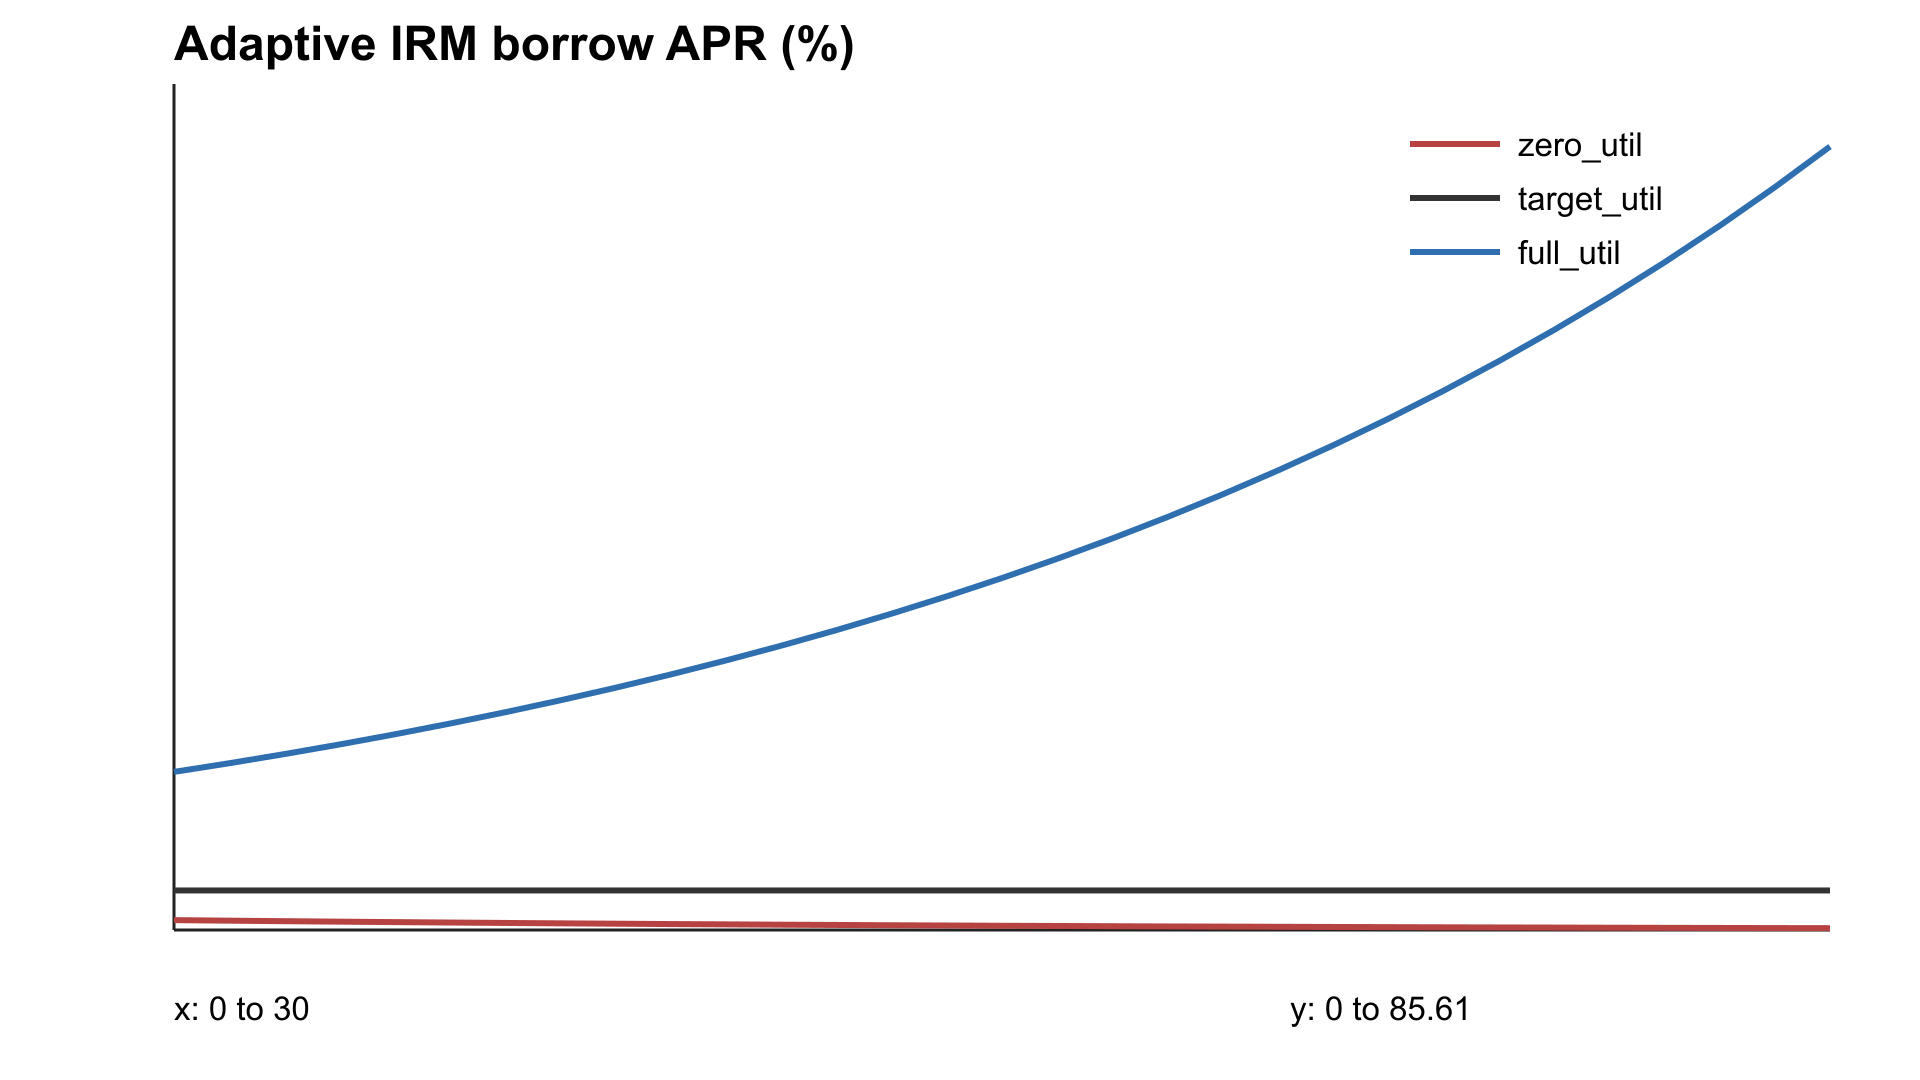
\includegraphics[width=0.78\linewidth]{simulations/figures/adaptive_irm.png}
\caption{Adaptive interest-rate paths for zero, target, and full utilization. The curve gives an immediate rate response; the target-rate anchor moves only when utilization persists away from target.}
\end{figure}

\begin{figure}[t]
\centering
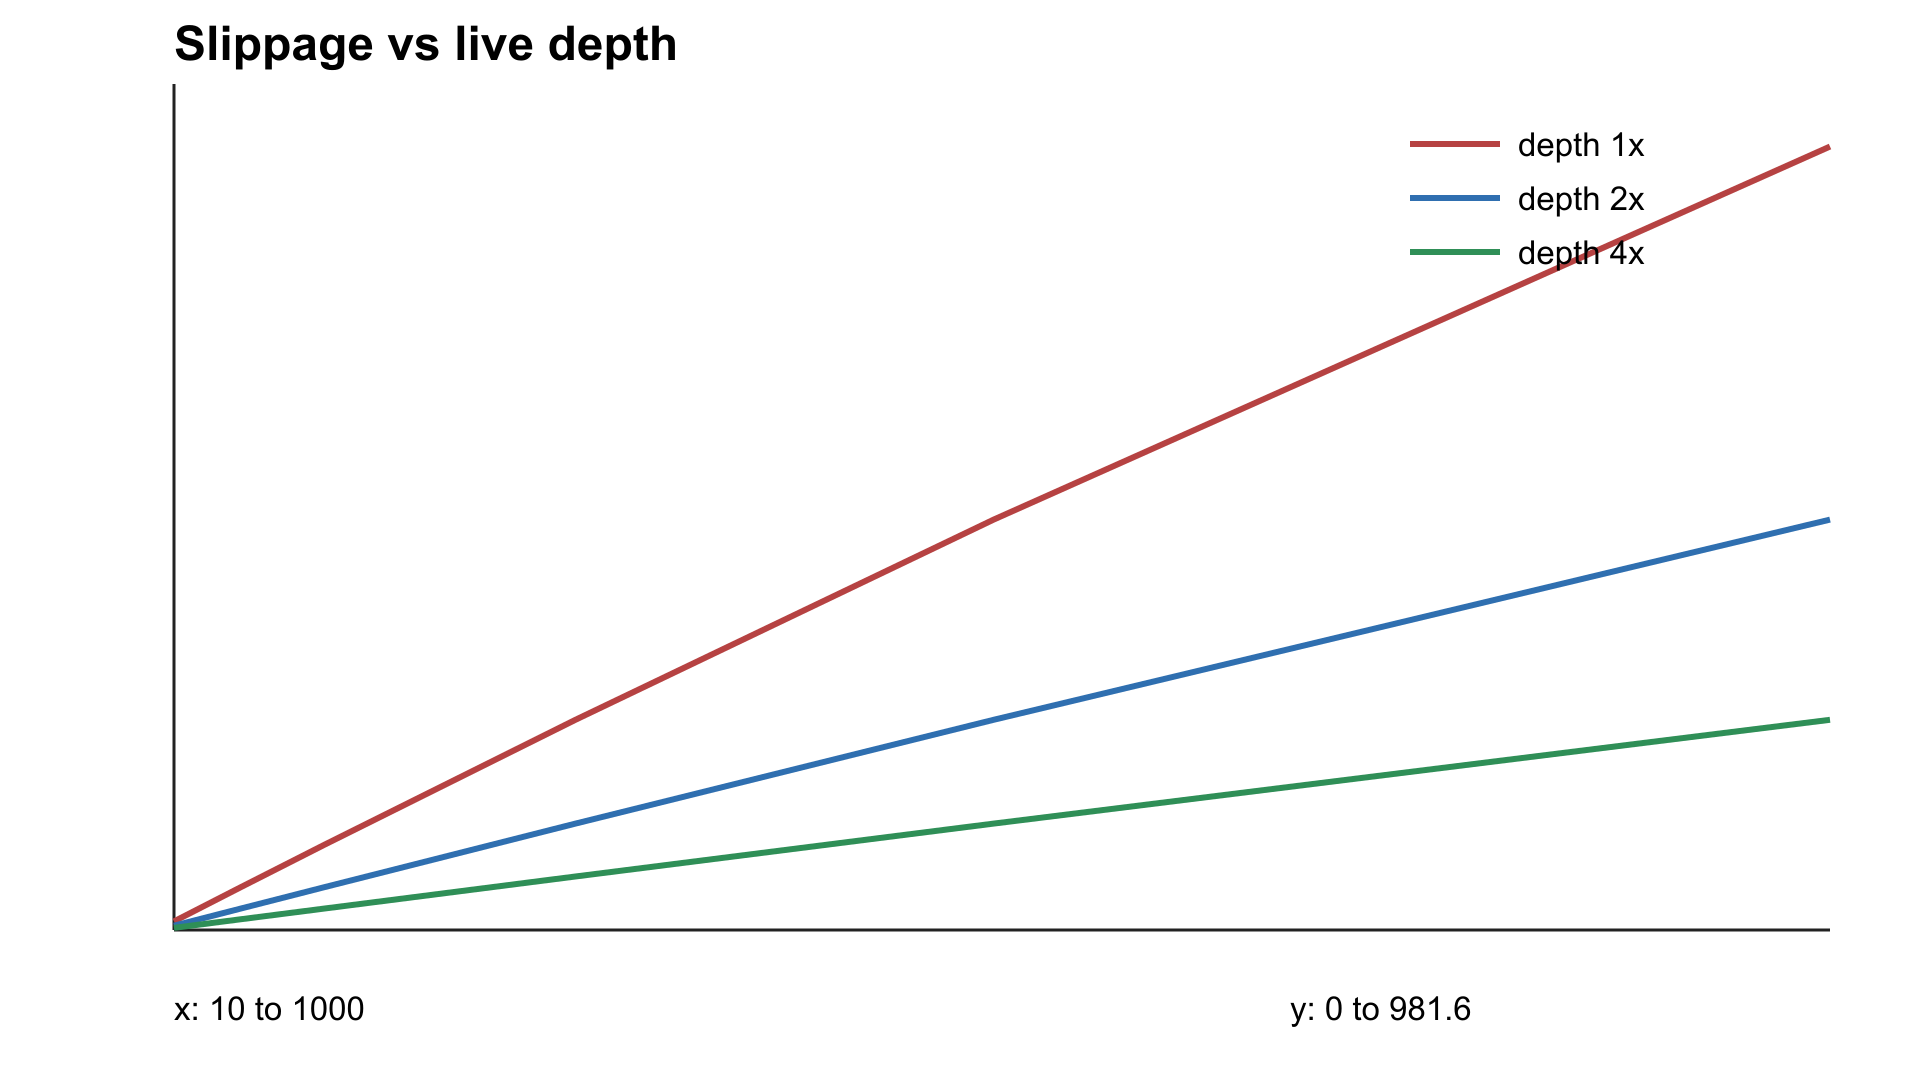
\includegraphics[width=0.78\linewidth]{simulations/figures/slippage_depth.png}
\caption{Constant-product slippage for the same trade size under larger live-depth coordinates. Balanced hLP live-depth changes preserve spot but reduce finite-trade price impact.}
\end{figure}

\begin{figure}[t]
\centering
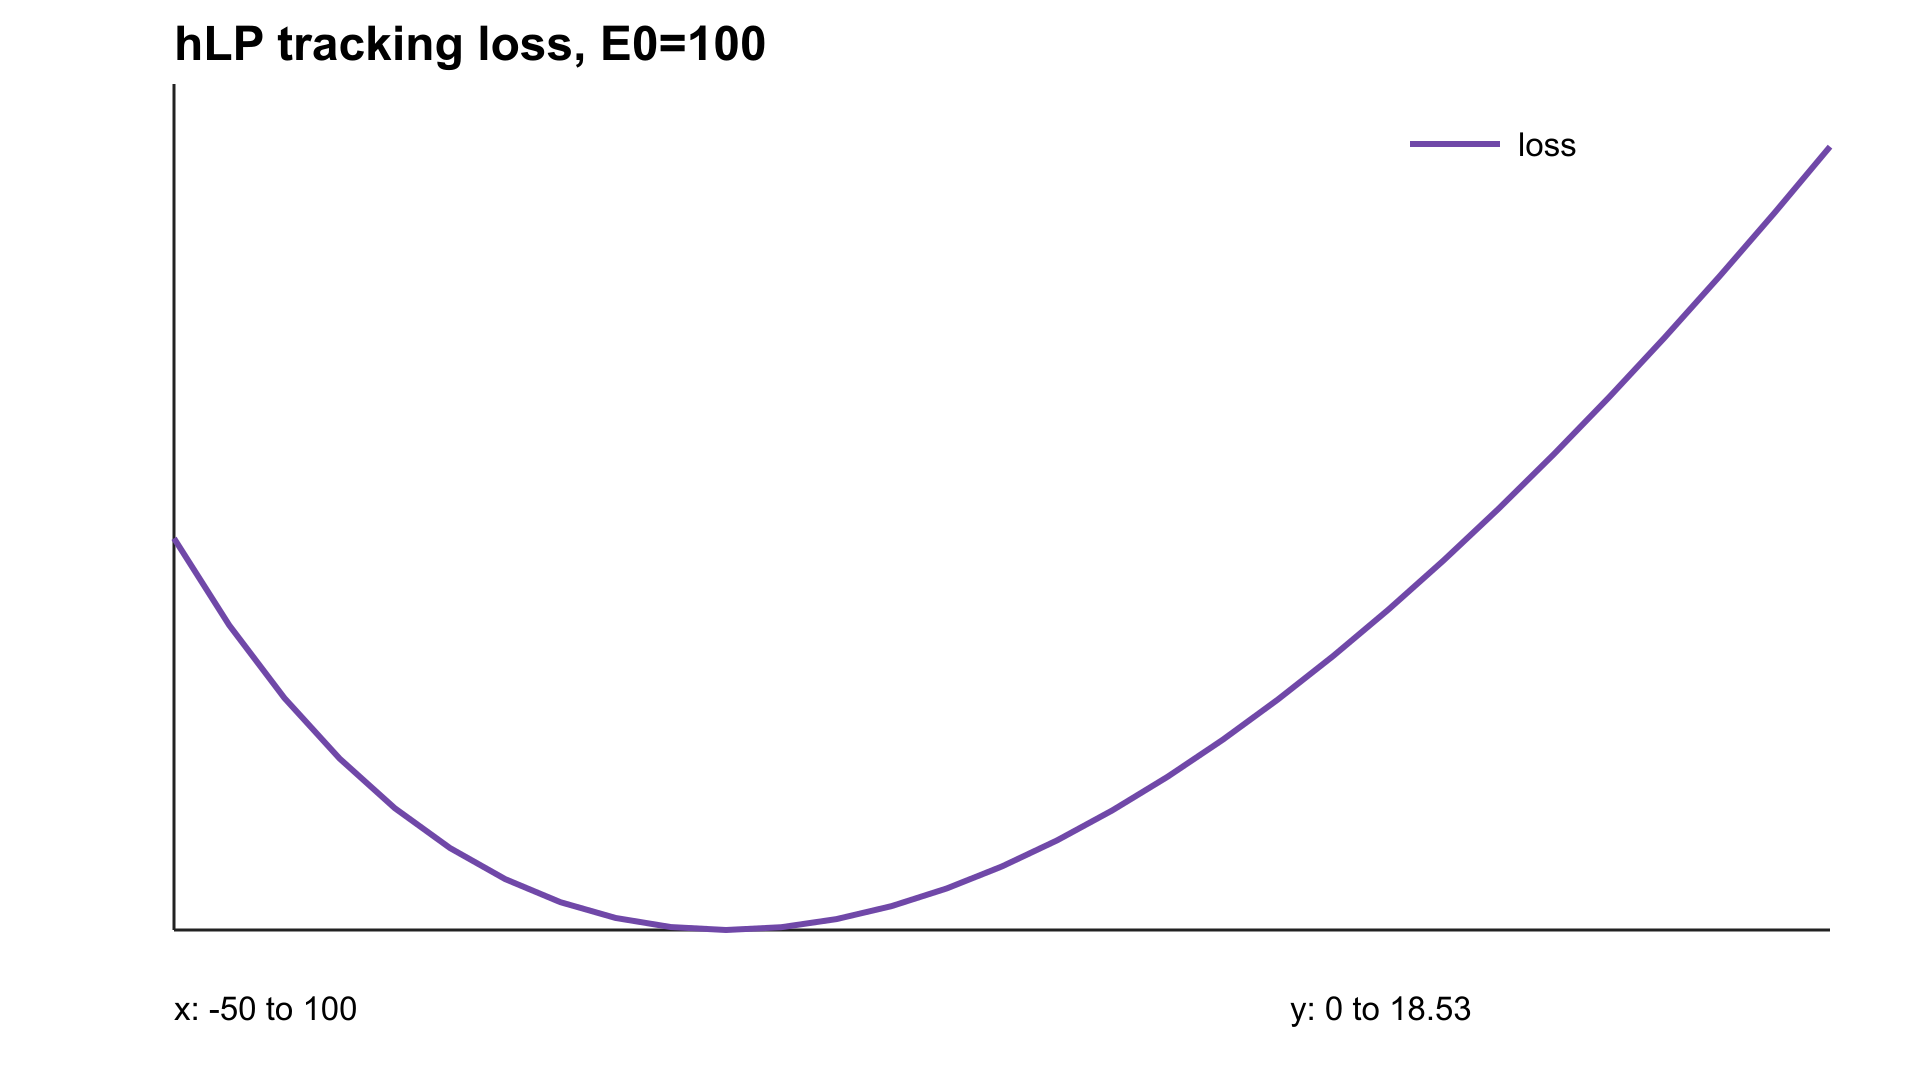
\includegraphics[width=0.78\linewidth]{simulations/figures/hlp_tracking_loss.png}
\caption{Discrete hLP tracking loss for $E_0=100$. The second-order shape is benign near zero and material for large price moves, motivating bounded just-in-time hLP updates.}
\end{figure}

Dusk has four important limitations.
\begin{enumerate}
  \item \textbf{Cash is stricter than live depth.} Synthetic hLP reserve can quote depth, but withdrawals and repayments require cash.
  \item \textbf{Local markets can still be bad markets.} Oracle-less does not mean riskless; it means the market's own depth, utilization, and risk books determine constraints.
  \item \textbf{Volatility creates operational load.} More volatile assets require more frequent hLP adjustment and stronger settlement guards.
  \item \textbf{Isolation contains losses but does not erase them.} Insurance and socialization define where residual losses go; they are not magic capital.
\end{enumerate}

The design is therefore best understood as a local mechanism for making long-tail leverage possible, not a universal guarantee that long-tail leverage is safe. Dusk replaces external oracle dependency with in-market accounting discipline. Its central bet is that this discipline is exactly what permissionless markets need.

\section*{Reproducibility}

Simulation sources are in \texttt{paper/simulations}. The scripts generate CSV and SVG artifacts for inspection without external APIs or notebook credentials. The LaTeX source is intentionally independent of those generated graphics so the paper remains buildable with a standard TeX installation.

\bibliographystyle{unsrt}
\bibliography{references}

\end{document}
